\begin{figure}[p]
\centering
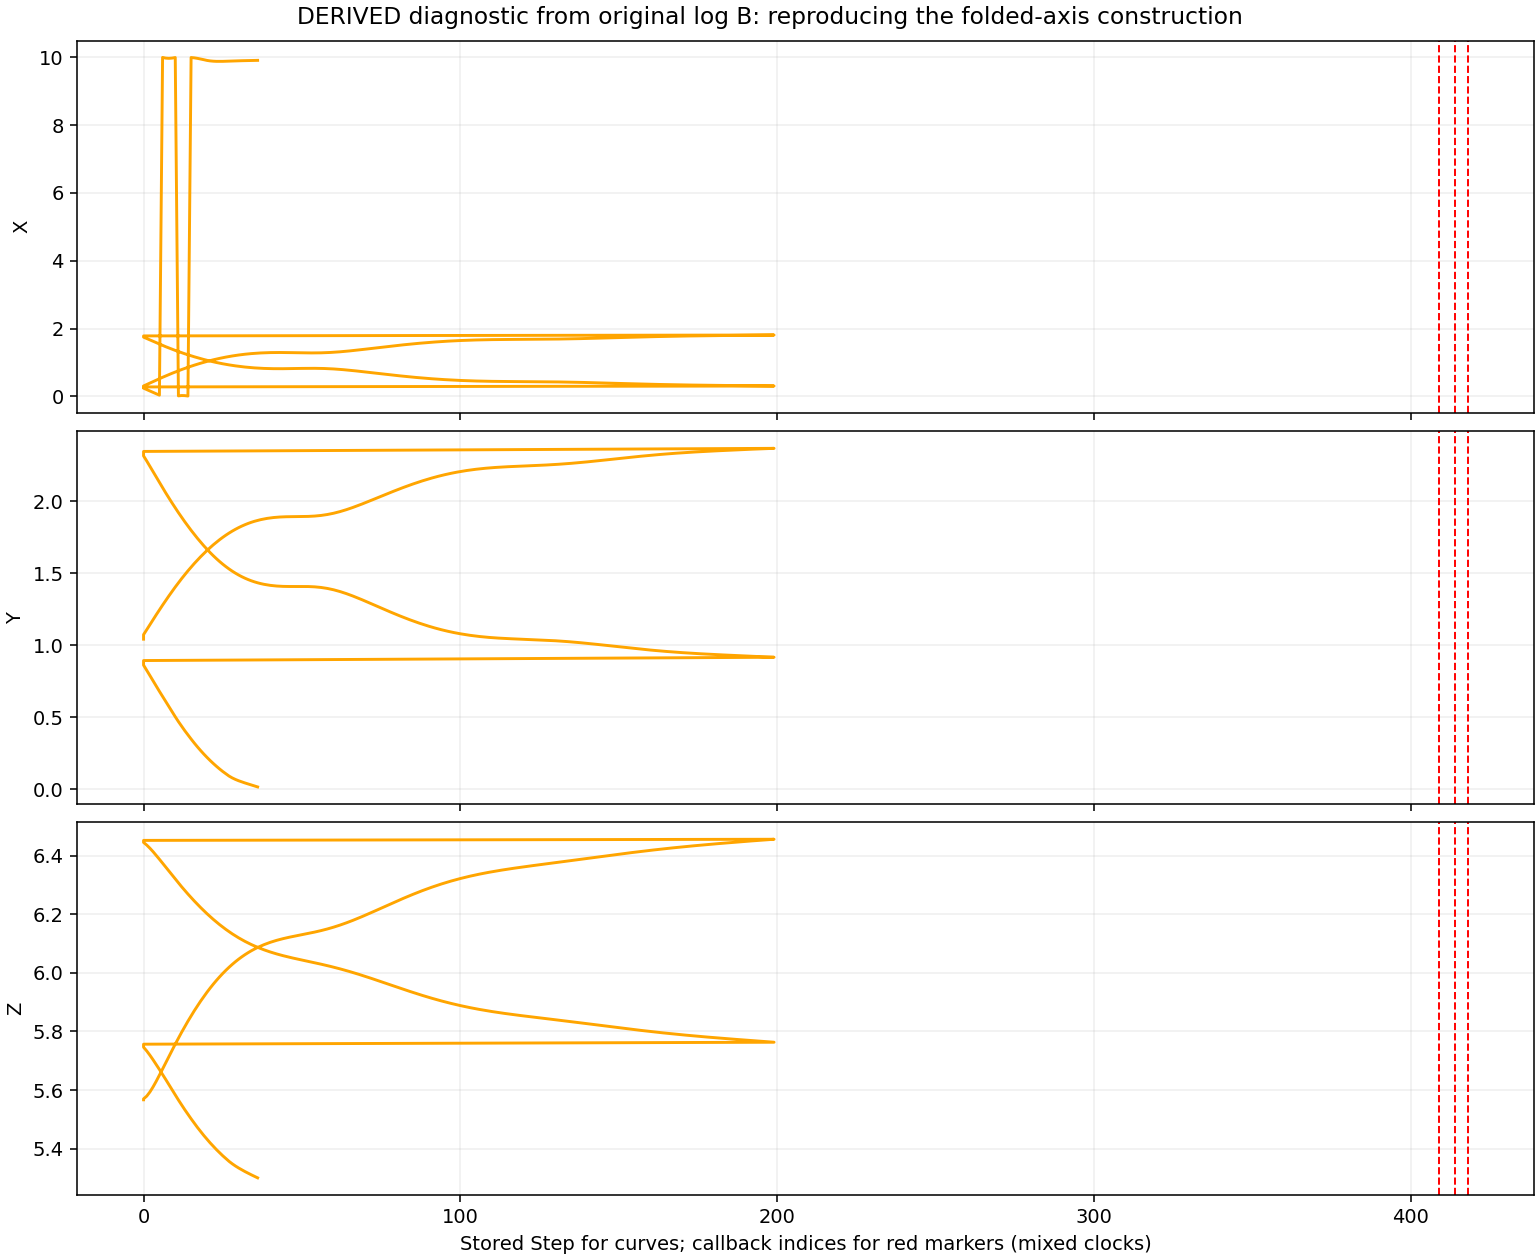
\includegraphics[width=\linewidth,height=0.70\textheight,keepaspectratio]{figures/F15_0.png}
\caption[Accepted diagnosis of the historical horizontal axes]{DERIVED from ORIGINAL log B, reused from Study 03. Repeated Step labels are used for the body 7 position traces while callback indices locate the three event markers. This recreates the misleading axis convention as a diagnostic; it does not repair the original chart or recover its exact generator. Lines joining label 199 back to 0 are drawing connections, not new trajectories. \cite{study03}}
\label{fig:F15}
\end{figure}
